\documentclass[pdftex,a4paper,titlepage,11pt]{article}

% Les packages de base pour le support du français
\usepackage[utf8]{inputenc}
\usepackage[T1]{fontenc}
\usepackage[english]{babel}

% La bonne police, sans serif, helvetica
\usepackage[scaled]{helvet}
\renewcommand*\familydefault{\sfdefault}
% \usepackage{palatino} % Palatino font
% \usepackage{lucidabr}

% Pour les liens/urls
\usepackage[colorlinks=true,linkcolor=black,citecolor=black,urlcolor=black,
filecolor=black]{hyperref}

% Le reste
\usepackage{verbatim}
\usepackage{graphicx}

% Pour ne pas avoir à mettre images/ devant les noms d'images...
\graphicspath{{images/}}
\usepackage{fullpage}
\usepackage{array}
\usepackage[absolute]{textpos}
\usepackage{framed}

% Pour les entêtes et les pieds de page
\usepackage{fancyhdr}
\pagestyle{fancy}
\usepackage{fancybox}

\usepackage{lastpage}
\usepackage{datetime}
\usepackage{multicol}
\usepackage{multirow}
\usepackage{eso-pic}
\usepackage{color}
\usepackage{sectsty}

% Pour avoir de beau listings
\usepackage{listings}
\usepackage{color}
\usepackage{textcomp}
\definecolor{listinggray}{gray}{0.9}
\definecolor{lbcolor}{rgb}{1,1,1}
\lstset{
	backgroundcolor=\color{lbcolor},
	tabsize=4,
	rulecolor=,
% 	language=bash,
	upquote=true,
	aboveskip={1.5\baselineskip},
	columns=fixed,
	showstringspaces=false,
	extendedchars=true,
	breaklines=true,
	prebreak = \raisebox{0ex}[0ex][0ex]{\ensuremath{\hookleftarrow}},
	frame=single,
	showtabs=false,
	showspaces=false,
	showstringspaces=false,
	identifierstyle=\ttfamily,
	keywordstyle=\color[rgb]{0,0,1},
	commentstyle=\color[rgb]{0.133,0.545,0.133},
	stringstyle=\color[rgb]{0.627,0.126,0.941},
}

\addtolength{\voffset}{-20pt}
\addtolength{\topmargin}{-6pt}
\addtolength{\headsep}{+12pt}
\addtolength{\footskip}{-4pt}
\addtolength{\textheight}{-23pt}
% \usepackage[top=1.5cm, bottom=5.5cm, left=2.5cm, right=2.5cm]{geometry}

% Pour le glossaire
% \usepackage[xindy, toc]{glossaries}
\usepackage[french]{nomencl}


%%Redefinition de commandes et autres utilitaires

%Ecart entre les colonnes
% \setlength{\columnseprule}{0.5pt}

% Définition des couleurs de l'ENSIB
\definecolor{darkBlueENSIB}{RGB}{0,52,120}
\definecolor{lightBlueENSIB}{RGB}{0,152,195}

\definecolor{fushiaENSIB}{RGB}{203,0,68}
\definecolor{orangeENSIB}{RGB}{255,109,34}

%Changement des couleurs des titres
\partfont{\color{darkBlueENSIB}{}}
\chapterfont{\color{darkBlueENSIB}{}}
\sectionfont{\color{darkBlueENSIB}{}\huge}
\subsectionfont{\color{darkBlueENSIB}{}\Large}
\subsubsectionfont{\color{darkBlueENSIB}{}\large}

\makeindex
% \makeglossaries
\makenomenclature

%Derniere page avec queue du poisson
\newcommand{\lastPage}{
	\newpage
	\strut
	\fancyhf{}
	\renewcommand{\headrulewidth}{0pt}
	\addtocounter{page}{-1}
% 	\AddToShipoutPicture*{\BackgroundPic{atos-logo-light.png}}
	\AddToShipoutPicture*{\BackgroundPic{Tux_n&b_half_1.png}}
	\newpage
}

% Modification du nom de la table des matières
% Ne semble pas fonctionner
% \renewcommand{\contentsname}{Sommaire}
% Titre pour le Glossaire/Index des noms
\renewcommand{\nomname}{Glossary}
%Separateur des dates
\renewcommand{\dateseparator}{/}

\renewcommand{\title}[1]{
	\vspace*{2cm}
	\begin{center}
		\Huge\textbf{{#1}}
	\end{center}
	\vspace{1cm}
}

\renewcommand{\author}[2]{
	\begin{center}
		\textbf{\Large{#1}}\\
		\normalsize{#2}
	\end{center}
	\vspace{0.3cm}
}

\newcommand{\school}[1]{
	\begin{center}
		\large{#1}
	\end{center}
	\vspace{1.0cm}
}


\newcommand{\supervisor}[4]{
	\begin{center}
		\begin{normalsize}
			{\bf#1}\\
			#2\\
			#3\\
			#4
		\end{normalsize}
	\end{center}
}

\newcommand{\clearemptydoublepage}{
	\newpage{
		\pagestyle{empty}
		\cleardoublepage
	}
}

\newcommand\BackgroundPic[1]{
	\put(0,-100){
		\parbox[b][\paperheight]{\paperwidth}{
			\vfill
			\centering
			\includegraphics[width=\paperwidth, height=\paperheight,
keepaspectratio=true]{#1}
			\vfill
		}
	}
}

%%
%% Redefinition des en-tetes et pieds de pages
%%
\fancyhf{}
\fancypagestyle{plain}

%%En tete
\lhead{\hspace{2.3cm}\large \textbf{Integrating PIGA-MAC into the Linux
kernel\\}}

% \chead{\large \textbf{Integrating PIGA-MAC into the Linux kernel\\}}

\rhead{\includegraphics[height=2.1cm, keepaspectratio=true]{Logo_ENSIB.png}}

%%Pied de page
\lfoot{}

\cfoot{\vspace{-0.8cm}\rule[0pt]{\textwidth}{0.1mm}\small
\ovalbox{\thepage/\pageref{LastPage}}}

\rfoot{\ddmmyyyydate \today}

%%
%% DOCUMENT
%%

\begin{document}

\begin{titlepage}
%%
%% Page de couverture
%%

\AddToShipoutPicture*{\BackgroundPic{Tux_n&b_half.png}}

\begin{center}
	\includegraphics[width=6cm, keepaspectratio=true]{Logo_ENSIB.png}
\end{center}

\vspace{0.5cm}

\begin{center}
	\fontsize{30}{30}\selectfont Integrating PIGA-MAC into the Linux kernel\\
	\vspace{2cm}
	\Huge 3rd year STI research project\\
	\Huge 2011 -- 2012
\end{center}

\vspace{2cm}

\begin{center}
	\begin{tabular}{rl}
		\hspace{7.5cm}
		\huge Teacher: & \huge Jérémy Briffaut\\[4pt]
		\huge Student: & \huge Timothée Ravier
	\end{tabular}
\end{center}

\vspace{0.5cm}

\begin{center}
\hspace{7.5cm}\includegraphics[width=5cm,
keepaspectratio=true]{Logo_SELinux.pdf}
\end{center}

\end{titlepage}

\newpage

~\thispagestyle{fancy}

\newpage

~

\vspace{1cm}
\addtocounter{page}{-1}

\section*{Acknowledgments}

~

I would like to thank Jérémy Briffaut for the many advices he gave me. This
project is based on his thesis and would not have been possible without his
work.

~

I would also like to thank Martin Peres as he introduced me to the PIGA concept
and kernel development.

~

\newpage

\tableofcontents

\newpage

\listoffigures

\newpage

\addcontentsline{toc}{section}{Glossary}

\nomenclature{\textbf{AppArmor}}{\textit{Application Armor:} a MAC mechanism
included in the Linux kernel}
\nomenclature{\textbf{DAC}}{\textit{Discretionary Access Control}}
\nomenclature{\textbf{HRU}}{Theorical model representing DAC systems}
\nomenclature{\textbf{IDS}}{\textit{Intrusion Detection System:} a device or
software that monitors network and/or system activities for malicious
activities}
\nomenclature{\textbf{IPS}}{\textit{Intrusion Prevention System:} an extension
of an IDS that also tries to block or prevent intrusions that are detected }
\nomenclature{\textbf{LSM}}{\textit{Linux Security Modules:} Hooks inserted in
the Linux kernel in order to implement modular access control}
\nomenclature{\textbf{MAC}}{\textit{Mandatory Access Control}}
\nomenclature{\textbf{MLS}}{\textit{Multilevel Security}}
\nomenclature{\textbf{MCS}}{\textit{Multi Categories Security}}
\nomenclature{\textbf{PaX}}{Linux kernel patch including support for
non-executable memory pages}
\nomenclature{\textbf{PIGA}}{\textit{Policy Interaction Graph Analysis}}
\nomenclature{\textbf{SELinux}}{\textit{Security Enhanced Linux:} a MAC
mechanism included in the Linux kernel}
\nomenclature{\textbf{SMACK}}{\textit{Simplified Mandatory Access Control
Kernel:} a MAC mechanism included in the Linux kernel}
\nomenclature{\textbf{TOMOYO Linux}}{A MAC mechanism included in the Linux
kernel}

\printnomenclature[3cm]

\newpage

\section*{Introduction} \addcontentsline{toc}{section}{Introduction}

This project is an integral part of my formation at the ENSI de Bourges, a
computer science and security french engineering school.

\bigskip

PIGA (Policy Interaction Graph Analysis) is an advanced Mandatory Access
Control mechanism designed to enforce security policy on a system. Just like
SELinux, PIGA does not directly prevent vulnerability exploitation, but
prevents any further action an attacker might attempt to perform on the system.

\bigskip

The current PIGA design faced unexpected problems and some of them are related
to the fact that the decision making code is located in userspace. That's the
main difficulty that we are trying to address with this kernel port. Among the
other problems that I will have to solve, they are multi-core and
multi-processor related issues. I will also try to improve performance and ease
of use while trying to port the complete PIGA feature set, which is an
ambitious goal.

\bigskip

I will begin with a short description of all currently available protections
for the main open source operating systems such as Linux distributions and some
from the BSD family. Then I will proceed to some PIGA reminders,
kernel/userspace implementation design. Finally, I will discuss some of the
problems I faced during those six months and potential solutions and
improvements for further development.

% FIXME Intro: performance ?
% Finally I will compare PIGA-Linux performance to kernel with either nothing,
% PaX, SELinux, ``classic'' PIGA enabled.

\newpage

\section{State of the art}

\subsection{Context and study limits}

%FIXME Add intro

There is a wide range of computer security problems, from hardware specific
ones to sotfware related flaws. New vulnerabilities are discovered every day
and they occur in every part of modern and complex operating systems. Current
mainstream systems are built around a core, or kernel, which controls and
abstracts hardware interactions that are provided to the applications. The
kernel has full control on the hardware and is often trusted to ensure that
each application running in userspace is separated from the others.

\bigskip

In this project, we will not focus on kernel security or kernel hardening
(despite the name PIGA-Linux). The main goal of PIGA is to go further than
SELinux, in order to enforce security properties on an operating system. So
I'll focus my study on mechanisms which allow a user or an administrator to
control permissions given to a program running on a computer. It could be
summarized as an advanced in-kernel control of userspace applications
behaviours.

\bigskip

Thus, I will use several restrictions to further constrain this study:
\begin{itemize}
	\item We are limited to the operating system; we do not take into account
interactions with an other system on the network for example;
	\item We want the solution to be as architecture independant as possible;
we should not require specific hardware design to work properly;
	\item As we do not take into account the underlying hardware, we do not
focus on hardware flaws either and therefore do not study hardware based
attacks (defective network card or driver...);
	\item We should focus on systems which have the source code available for
study.
\end{itemize}

\smallskip

Most of current operating system are using an access control design to ensure
minimal security, seperation and control on user's activities. They were
introduced to limit the effects of an attack against the operating system. But
this limited control does not prevent complex attack scenario, such as the
compromission of a service which was given adminstrative rights on the system.
\cite{inevitabilityoffailure1998} describes in details most of the problems
current operating
systems are still facing nowadays.

\bigskip

Generally speaking, we lack a global, truly enforced, system wide security
mechanism. More than simple checks in interactions between kernel and
userspace, it's the whole interaction set on a system that need to be
controlled.

\bigskip

First I'm going to detail the objectives an operating system has to achieve.
Then I will discuss theorical models and their implementations in modern
systems.

\bigskip

In this study, I will refer to files (and others ressources such as sockets) as
objects, and to program as subjects, whether or not they are directly
controlled by a real human user on the system.

\subsection{Generality}

\subsubsection{Security objectives}

% FIXME find the paper on security objectives
There are three main objectives generally defined in computer security articles
and governmental processes \cite{tcsec1986}. An operating system has to provide
means to ensure they can be enforced:

\bigskip

\textbf{Confidentiality:}
Information must only be available to users who need it and have the
corresponding privilege. Example: a user should not have access to other users
passwords, files or secrets; classified information should not be available for
unclassified users to read.

\medskip

\textbf{Integrity:}
The system must remain in coherent state. Example: important information such
as passwords, which programs are installed and their content, configuration
files, should not be alterable by unprivilege users.

\medskip

\textbf{Availability:}
The system must remain stable, reactive and usable. Programs have to function
properly. Added security controls should limit as little as possible legitimate
system functionnality and programs.

\bigskip

I will focus on the first two properties, which are confidentiality and
integrity. Attack scenario such as Denial of Service will therefore not be
taken into account as their goal is to limit a system disponibility. Future
references to security objectives will include only those two.

\bigskip

However, a security solution should not turn a working system to an unsable one
and thus it can not have a high ressource footprint. I'll try to limit the
impact on performance of the chosen solution.

\subsubsection{The principle of least privilege}

The process to make the first step toward the previously discussed objectives
is based on the principle of least privilege. It involves two steps:
\begin{enumerate}
	\item make sure each major program functionnality is divided into smaller
program (generally depending on their ressource needs);
	\item restrict the rights of each program to the smallest set of
permissions needed for it to function well.
\end{enumerate}

\smallskip

The most common examples are the postfix and qmail mailer daemon. They are
divided in several programs and communicate using files or SystemV IPC. There
is a network facing program, a user facing program and the code running under a
privilege user is therefore severely limited, which, as a side effect, improves
it's auditability. This way a vulnerability will only impact one program which
has a limited permission set. It would require several flaws in each different
part to gain enough privilege to affect the system.

\bigskip

Generally speaking, a program should not have acces to a ressource if it
doesn't use it, even if it isn't a confidential ressource.

\bigskip

On modern operating system, this separation is often enforced using different
user accounts with different capabilities. There is an administrator which has
all rights on the system, several unprivileged account for regular users,
and network enabled accounts for services such as the web server.

\bigskip

However, few programs are well designed enough to benefit from this rule. It
also doesn't provide a solution in case of program compromission so this isn't
enough to enforce security objectives.

% Il faut cependant noter que ce principe ne constitue pas une démarche
% exhaustive permettant d'assurer des objectifs de sécurité.

\subsubsection{Who/what do I need to trust?}

Every design made to secure an operating system has to rely, at some point, on
one of it's components (either a hardware one, a software one, or both). This
component is trusted to be safe and hardened against attacks. This is
summarized in this list:

\begin{itemize}
	\item Trust all the software to abide by a security policy while being
aware that the software is not trustworthy;
	\item Trust all the software to abide by a security policy and the software
is validated as trustworthy (by static analysis, unit testing, branch analysis);
	\item Trust no software but enforce a security policy with mechanisms that
are not trustworthy;
	\item Trust no software but enforce a security policy with trustworthy
hardware mechanisms.
\end{itemize}

\smallskip

Standard security models are in the first category whereas most of the one I
will present later are in the third and forth ones.

\bigskip

Testing the whole feature set of an operating system is a tedious task. This is
even harder if we consider the various architectures,hardware diversity and the
complexity involved in the design of core pieces of an operating system such as
the kernel. Some software, such as the QNX operating system
\cite{qnxoperatingsystem}, have had
intensive testing, a controlled design and are certified as conforming to
strict criteria like the Common Criteria \cite{commoncriteria}. Those systems
are part
of the
second category. However, the source code for those operating systems are not
freely available so I will not detail them much further.

\bigskip

The Figure \ref{INTELTXT} \cite{inteltxt} shows an example of hardware based
integrity control,
with corresponds to the fourth category. Its goal is to verify the signature
of critical components in the system to make sure that they have not been
tampered with before boot. If the check fails, the system is unable to boot.

\begin{figure}[h]
	\centering
	\includegraphics[scale=0.70]{techrefresh-info-txtfull.png}
	\caption{Intel Trusted Execution Technology}
	\label{INTELTXT}
\end{figure}

\smallskip

The Linux Integrity Subsystem \cite{linuxima} is an other example of hardware
assisted integrity control, involving a Trusted Platform Module (TPM) which
stores cryptographic keys. However this approach is rather complex and protects
only from some off-line based attacks which are not detailled in this study.

\bigskip

It should be noted that both of those mechanisms only provide detection and
can not prevent an intrusion or corruption from happening.

\subsection{Access control models}

Several Access control models have been implemented in modern operating systems
to achieve the objectives mentioned previously. I'll detail those models in
this section.

\subsubsection{Discretionary Access Control (DAC)}

The Discretionary Access Control model give each user full control over the
files and other system objects it owns. The control is left at the discretion
of the user, and most of the time this is also the identity impersonated by an
attacker.

\bigskip

Applications ran by this user are also given the same control, and most of the
time they have too many privileges. For example, Firefox can access any file
stored in the user home directory, including the user ssh private key.

\bigskip

DAC based operating systems are also often vulnerable to the confused deputy
problem \cite{confuseddeputyproblem}. In this scenario, a privileged
application is tricked by an underprivileged one into revealing information or
acting in a particular way which wasn't intended in the first place.

\bigskip

This model can not ensure confidentiality or any other complex property as for
example a user give grant access to other users on confidential information he
has access to. DAC is to be considered as being part of the first category, in
which no clear policy is enforced on the system. \cite{hru1976protection}
further describes why a DAC based system will not be able to ensure security
properties.

\subsubsection{Mandatory Access Control (MAC)}

The reasons behind the increassing necessity to use Mandatory Access Control
are fully described in \cite{inevitabilityoffailure1998}. They are partialy
summarized in this example: Browers (and related plugins) are considered as the
most used attack vector for conventionnal desktop computers. With classic DAC,
a user's Firefox process would have the same privilege as any other program ran
by this user. So Firefox would be able to read the user's private ssh keys
generally stored in their base directory and send it to a remote attacker.

\bigskip

The MAC philosophy is to enforce the principle of least privilege to every
program on an operating system. Firefox would then not have the required
permissions to acces those keys, as only the ssh daemon would be able to do so.
The consequences of users making bad choices or mistakes, while managing the
permissions given to his files for example, are also severly limited in a MAC
environment.

\bigskip

MAC mechanisms are based on clear distinctions between the user (its
applications) and the process responsible for grating or denying permissions.
This ``process'' can be implemented as an other application but generally
require cooperation from the kernel. Its goal is to ensure that a set of rules,
the security policy, are enforced on a system.

\bigskip

Using MAC, we can build a policy enforing the least privilege design by
starting with a base policy denying acces to everything, and progressively
allowing applications to use the ressources they need. In terms of trust, MAC
can be categorized in the third and forth ones which means not trusting
applications to behave properly and ensuring that another mechanism, software
or hardware based, will control them.

\subsubsection{Capability-based security}

Capability-based security is a concept which gives each subject or process a
restricted set of permissions on critical ressources. A process will never be
able to gain more permissions, and it can only give the permissions it already
owns to its children. As with those restrictions every process on the
system would only lose capabilities, such operating systems implements
capability exchange to allow granting of selected capabilities. There are only
a few operating systems implementing such design \cite{capabilitycapsicum}.

\bigskip

The Linux kernel implements a similar but very basic concept of capabilities to
limit the need of binaries with the setuid flag. This flag allows binaries to
be run under the uid or identity of the binary owner and is often used to allow
users to run programs which require root privileges. In this case, capabilities
allow the administrator to grant a process the access to a restricted set of
system ressources such as binding on TCP port under 1024 while keeping the
process runnning under an underprivileged user. Those capabilities can not be
transfered to other processes.

\subsubsection{Multilevel Security and Multi Categories Security (MLS \& MCS)}

The multi-level and multi-category security model enable us to achieve goals
such as integrity and confidentiality. Objects and subjects are separated in
several category or security level and rules are set up to limit interactions
between those levels or category.

\bigskip

\textbf{Bell-LaPaluda:} This model \cite{BLP} tends to preserve confidentiality
of
information as it only allows a subject to write information to a superior or
equal level of confidentiality, and read information from an equal or inferior
level. The several disadvantages in this model are the lack of integrity control
and distinctions between too subjects with the same confidentiality level.

\begin{figure}[h]
	\centering
	\includegraphics[scale=0.5]{bell-lp}
	\caption{The Bell-LaPadula Model}
\end{figure}

\bigskip

\textbf{Biba:} As opposed to the previously described model, it's integrity
control that's being enforced by the Biba design \cite{Biba}. Only modifications
in an inferior or equal level and reads from a superior or equal level are
allowed.

\begin{figure}[h]
	\centering
	\includegraphics[scale=0.5]{biba}
	\caption{The Biba Integrity Model}
\end{figure}

\bigskip

Those relatively simple security model can not enforce more than a single
security property at the same time. They also raise the problem of over
classification as in the Bell-LaPadula model, information can only get more
classified, and its declassification require the intervention of a trusted
user. This partially compromise the model as it can not function without
external intervention. In fact, those models can be applied to reduced sections
of an operating system to provide local integrity and confidentiality checks.

\subsubsection{Role Based Access Control (RBAC)}

Role Base Access Control is an administration model to simplify the management
of MAC enabled operating systems. It allows to regroup desired set of
permissions into several roles and assign roles to users. For example, the
user, admin, web\_admin roles could be defined so an user could be given
control over the web server without requiring full acces as in root or admin
access to the server. This also allows the administrators to easily grant and
remove a large group of various permissions to an user, thus improving
management.

\subsubsection{Type Enforcement}

The Type Enforcement model is based on a reference monitor and full labelling
of system ressources. A security context is associated to each object and
subject and every interaction between any subject or by a subject on an object
is controlled by the reference monitor. Most of the time, decisions are based
on a policy which is enforced on the system by a trusted element, which is
often sotfware based such as the operating system kernel.

\bigskip

The only allowed interactions are those defined in the policy and any other
access is denied by the reference monitor. This model require the administrator
to grant only the required permissions to selected subjects and to chose a
security context for every file on every storage used by a system.

\subsection{Available solutions to enforce Mandatory Access Control}

This section will detail the different implementations of security models in
some operating systems. I decided to concentrate my study on systems where the
source code is freely available for study: Linux and the BSD family. This
section is based on the detailled summary on page 86 of
\cite{theseJBriffaut} and \cite{maccomparison}. As of today, the first four
solutions are available in the upstream Linux kernel as Linux Security Modules.

\subsubsection{Simplified Mandatory Access Control Kernel (SMACK)}

The SMACK model \cite{schaufler2008simplified} is explicitly focused on easy
administration and easy setup. It is based on security labels that are given to
every objects and subjects on a system. Access control is enforced by storing
rules inside the security labels. Several special labels allow read only or
write only support for example. 

Userspace support in applications is not required to function properly, but
some scripts are provided to simplify setup and management.

\begin{list}{}{}
 \item \textbf{Constrains for the administrator:} No centralized policy or
label management. Must carefully setup every label on the system to avoid
mis-labelling. Does not advertise audit features.
 \item \textbf{Advantages:} Easy to setup as there isn't any particular tool
required. Presented as simple, according to the author, as compared to SELinux
for example.
\end{list}

\subsubsection{TOMOYO Linux}

The TOMOYO Linux tool \cite{tanaka2003access} \cite{harada2004task}
\cite{harada2005towards} is a project enabling users and administrators to
easily build a security policy by a ``try and learn'' mechanism. It focuses on
clear policy generation, path base control and process history. It also
features per application firewall, application behaviour audit, confined
environment for remote users for example and a simple RBAC management. However,
the current version integrated into the Linux kernel is not complete and cannot
provide the full functionnality.

\begin{list}{}{}
 \item \textbf{Constrains for the administrator:} No initial policy
provided, require manual tweaks to be really efficient
 \item \textbf{Advantages:} Learning mode available, audit tools, progressive
setup.
\end{list}

\subsubsection{Application Armor (AppArmor)}

The AppArmor security module provide application centered control. It enforces
capabilities and access restrictions and features a learning mode which logs
access and simplify profile configuration. It was designed to be easier to setup
than SELinux.

\begin{list}{}{}
 \item \textbf{Constrains for the administrator:} No global policy. Must setup
each program separately.
 \item \textbf{Advantages:} Learning mode available, some profile are provided
by distributions for widely used softwares.
\end{list}

\subsubsection{Security Enhanced Linux (SELinux)}

SELinux is MAC mechanism implemented in the Linux kernel as a Linux Security
Module \cite{lsm2002linux}. Originally developed by the National Security
Agency (NSA), it features type enforcement based MAC, RBAC management, MLS and
MCS support. It is based on security contexts associated with each objects on
the system, and a reference monitor implemented in the Linux kernel. Just like
any other LSM based access control, SELinux checks every system call for
compliance to a set of previously loaded policy. Every choice is made
independantly, ensuring SELinux is stateless thus ignoring covert channels and
indirect interactions.

\begin{list}{}{}
 \item \textbf{Constrains for the administrator:} The full set of allowed
interactions as to be described in a specified language to create the policy.
Proper testing must ensure that every application can access the ressources
they need. File systems must be able to store security context as an extended
attribute, preventing the use of old or exotic ones. Network operations (NFS
shares) are challenging and require external control.
 \item \textbf{Advantages:} Fine-grained confinement of subjects on a
system; available in several mainstream distributions and well-tested in the
Linux kernel; a reference policy is available.
\end{list}

\subsubsection{Policy Interaction Graph Analysis - Mandatory Access Control
(PIGA-MAC)}

PIGA is a concept with a collection of associated tools made by Jérémy Briffaut
as a proof of concept for his PhD thesis and further enhanced later with the
help of the SDS team from the LIFO laboratory and ENSIB students to produce
PIGA-OS. The PIGA-OS operating system won the Sec\&Si challenge organized by
the french National Research Agency (ANR) \cite{pigaosdefisecurite2011}
\cite{pigaproperty2010}. It's goal is to enforce security properties on a system
thanks to an activity description language and a compiler to obtain sequences of
SELinux interaction that are infringing those properties. This improvement could
be simplified as being a statefull SELinux implementation and is able to detect
covert channel exploits.

\begin{list}{}{}
	\item \textbf{Constrains for the administrator:} Knowledge of
the activity description language and SELinux is required. The PIGA policy
generator is performance hungry, but it is a one time operation.
	\item \textbf{Advantages:} Fine-grained control over on going interaction.
SELinux advantages.
\end{list}

\subsubsection{PaX \& grsecurity}

grsecurity \cite{grsecuritywebsite} is another implementation of the MAC and
RBAC models. It also features Access Control Lists and trusted path execution,
ensuring the binaries on the system can not be modified by untrusted users.
Often associated with PaX witch is a Linux kernel patch, it brings heavy
restrictions to the rights given to standard users and access to memory pages.

\begin{list}{}{}
	\item \textbf{Constrains for the administrator:} Several program do
not work with the PaX restrictions. The trusted execution of programs require
carefull administration and policy design.
	\item \textbf{Advantages:} Advanced memory protection, rule learning
feature, simplier design compared to SELinux.
\end{list}

\subsubsection{W\^{}X \& TrustedBSD}

The Trusted BSD project \cite{trustedbsdproject} has added a feature
similiar to PaX called W\^{}X to enforce separation between executable and
writable memory pages on FreeBSD. Audit capabilities, Access Control Lists and
several MAC mechanisms were also added. As I'm not familiar with *BSD operating
systems, I will not detail this section much further.

% \subsubsection{PIGA-SYSTRANS ou contextd}
%
% Contextd est un démon chargé de coordonner différents mécanismes de sécurité
% sur un système Linux. En effet, dans toutes les solutions décrites
% précédemment,
% les programmes se voyaient attribuer les droits dont ils avaient besoin, pour
% toujours. Une application utilisant ponctuellement le réseau se voyait
% attribuée
% le droit définitif d'utiliser un port. Contextd introduit la notion de domaine
% (web, impôts, ...) lié à une activité particulière de l'utilisateur. Les
% programmes surveillés n'ont le droit de faire que ce qui leur est autorisé
% dans
% le domaine courant.
% \begin{list}{}{}
%  \item \textbf{Contrainte pour l'administrateur:} Maîtrise de SELinux, PIGA.
% Rédaction et test des règles exhaustives pour faire fonctionner les programmes
% avec contextd. Certains programmes nécessitent des modifications, surtout
% lorsque ceux-ci ont un comportement inter-domaine.
%  \item \textbf{Avantages:} Presque la plus fine implémentation du principe de
% moindre privilèges.
% \end{list}

% Pax = sécurité automatique
% SELinux, GrSec = MAC qui contrôle les accès directs
% PIGA = contrôle les accès indirects
% iptables contrôle le trafic réseau
%
% contextd = chef d'orchestre + changement dynamique des règles des autres
% mécanismes de protection pour adapter les permissions au domaine
% d'utilisation.
%
% Chercher tous les systèmes de MAC/DAC/RBAC,...
%
% Classer les MAC en fonction du travail à faire par l'administrateur ? en
% fonction d'où ils agissent ? par rapport à la logique interne (stateless ou
% statefull) ?

\newpage

\section{Development and test environment}

PIGA features are intrinsically linked to SELinux features so the choice of
development environment was limited. The main GNU/Linux distributions
supporting SELinux are:

\begin{itemize}
	\item Red Hat Enterprise Linux \cite{rhelwebsite}, CentOS
\cite{centoswebsite}, Scientific
Linux \cite{scientificlinuxwebsite}, Fedora \cite{fedorawebsite};
	\item Gentoo \cite{gentoowebsite} with the Hardened Gentoo project
\cite{gentoohardenedproject}.
\end{itemize}

\smallskip

As PIGA-OS is based on Hardened Gentoo, I chose to stick with this distribution
as the primary development environment.

\subsection{Hardened Gentoo}

The Hardened Gentoo Project has taken upon the goal of building a completly
secure operating system from the ground up. To achieve this goal, several
particularities have been selected:
\begin{itemize}
	\item a linux kernel with the PaX \& grsecurity patch;
	\item a carefully crafted configuration and several restrictive
compilation options;
	\item a modular SELinux policy based on the reference policy.
\end{itemize}

\smallskip

The first step of this project was to setup a virtual Hardened Gentoo
development environment. I used the well written Gentoo SELinux Handbook
available at \cite{gentooselinuxhandbook}.

\bigskip

The Gentoo choice was also driven by the fact that I had to understand most of
the building process in order to make it work properly. This constrain was
actualy a benefit as I needed a clear view on how SELinux works and how do I
manage it.

\subsection{QEMU, KVM, libvirtd and the Virtual Machine Manager}

In order to ease the development process, I used some KVM and QEMU special
features. The Virtual Machine Manager also provided me with all the tools
required to deploy QEMU/KVM virtual machines more easily.

\subsubsection{Using an host compiled kernel}

QEMU enabled me to use an externaly (as in: not on a virtual drive) compiled
kernel. It saved me a lot of time in kernel compilation as I was able to do it
on the host system instead of the virtual one. As the host and the virtual
machine architecture matchs (x86\_64), there was no cross-compilation involved
and I simply used this kernel into the Gentoo virtual machine.

This option is enabled with the corresponding arguments added to the qemu
command line:

\begin{lstlisting}
qemu-kvm ... -kernel path/to/bzImage -append root=/dev/sda1 ro quiet
\end{lstlisting}

\subsubsection{Debuging a kernel with QEMU and gdbserver}

One of the many useful feature in the QEMU emulator is the ability to debug a
kernel running inside a virtual machine thanks to the gdbserver program. In
order to use it, you have to add this argument to the qemu command line, where
1234 is the port you want it to listen to:

\begin{lstlisting}
qemu-kvm ... -gdb tcp::1234
\end{lstlisting}

\subsubsection{libvirtd XML configuration}

To simplify network setup and management for virtual machines, I choosed to
use libvirtd and the graphical user interface called virt-manager which
stands for Virtual Machine Manager. The libvirtd daemon uses XML files to
store virtual machines configurations. This is the example configuration I
used, including the previously discussed QEMU features:

\begin{lstlisting}
<domain type='kvm' xmlns:qemu='http://libvirt.org/schemas/domain/qemu/1.0'>
  <name>Gentoo_projet</name>
  <memory>2097152</memory>
  <vcpu>1</vcpu>
  <os>
    <type arch='x86_64' machine='pc-0.14'>hvm</type>
    <kernel>linux-2.6.39-hardened-r8/arch/x86_64/boot/zImage</kernel>
    <cmdline>root=/dev/sda1 ro quiet</cmdline>
    <boot dev='hd'/>
  </os>
  ...
  <devices>
    <emulator>/usr/bin/qemu-kvm</emulator>
    <disk type='file' device='disk'>
      <driver name='qemu' type='raw'/>
      <source file='gentoo_projet.img'/>
      <target dev='hda' bus='ide'/>
      <address type='drive' controller='0' bus='0' unit='0'/>
    </disk>
    <interface type='network'>
      <model type='e1000'/>
      ...
    </interface>
    ...
  </devices>
  <qemu:commandline>
    <qemu:arg value='-gdb'/>
    <qemu:arg value='tcp::1234'/>
  </qemu:commandline>
</domain>
\end{lstlisting}

% \subsubsection{Constrains related to the QEMU emulator}

% Finally, I had to ensure that the modifications I would introduce in the
% kernel would not prevent the use of PIGA in a virtual environment, thus the
% use of QEMU.

% \subsection{Related tests}

% This virtual environment allowed me to test several of the available solutions
% (SMACK, TOMOYO...).
% J'ai ainsi créé une machine virtuelle pour chaque solution et j'ai testé les
%scénarios d'attaques et la réponse que pouvait apporter un administrateur à ces
%scénarios.
% Violation d'intégrité:
% Violation de confidentialité:
% \subsection{Résultats}
% Tableau comparatif avec le DAC...

\newpage

\section{PIGA-Linux}

\subsection{What does PIGA do?}

PIGA's first objective was to detect any malicious activity on a system. To
achieve this goal, PIGA is built on top of an other MAC (only grsecurity
and SELinux in its current form).

\bigskip

Each MAC implementation defines operations or interactions performed on a
system by userspace programs (read, write...). PIGA  builds a graph with the
MAC defined interactions in order to obtain an exhaustive view of all the
interactions and sequence of interactions that are allowed on a system.

\bigskip

The language defined in \cite{theseJBriffaut} is designed help administrators
represent security properties. Administrators can use this language to define
which properties they want to ensure on a selected system (program binaries
integrity for example). Then, the PIGA-pol tool will generate the full list of
sequence of interactions infringing the security properties from the
interaction graph previously generated.

\bigskip

This will ensure that no cover-channel or alternative way can be used to
exploit a weakness in the MAC policy. \cite{theseJBriffaut} contains a full
description of PIGA features.

\bigskip

The Figure \ref{PIGAARCHI} details the process to generate the signature
database from both an access control policy and a detection policy. Those
signatures can then be used to enforce access control on a system and report
access errors or warnings.

\begin{figure}[h]
	\centering
	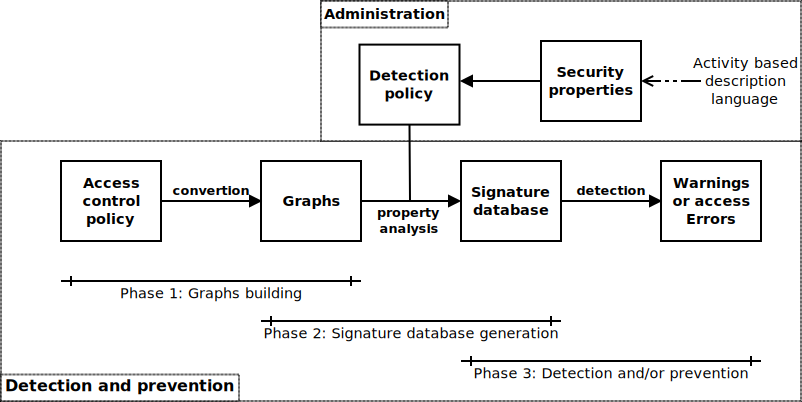
\includegraphics[scale=0.37]{modele_generale_en.pdf}
	\caption{The process to enable PIGA control}
	\label{PIGAARCHI}
\end{figure}

\subsection{Why porting PIGA to Linux?}

The PIGA concept gave birth to several components such as the PIGA-IDS/IPS,
which is an userspace daemon written in Java. It was developped as a proof of
concept and turned into a fully working IPS for the PIGA-OS project
\cite{pigaosdefisecurite2011}. Its userspace design led to some limits and
raised unexpected problems for network related interactions. It also introduced
several additionnal context switches for each system call and had a limited but
mesurable impact on the system performance.

\begin{figure}[h]
	\centering
	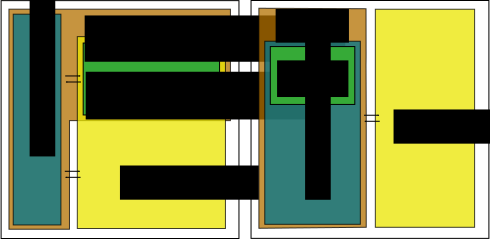
\includegraphics[scale=1.1]{piga_evol.pdf}
	\caption{From PIGA-IDS/IPS to PIGA-Linux}
	\label{PIGAEVOL}
\end{figure}

\smallskip

From a security point of view, the process making the decission to allow or
deny access what located in userspace and thus was more vulnerable to
conventionnal attacks.

\bigskip

Several of those problems could be solved more easily by moving the decision
making process into the kernel.

\subsection{Objectives}

The following objectives (and implementation order) were layed out with Jérémy
Briffaut at the begining of the project:

\begin{enumerate}
	\item Implement a basic decision making algorithm in the kernel
	\item Create userspace tools to load a PIGA policy into the kernel
	\item Optimize the policy storage into the kernel to handle large policy
(more than three hundred thousand signatures) in order to make this useful in
the real world
	\item Implement remaining PIGA-IDS and PIGA-IPS fonctionnality (conditionnal
policy, process based signatures, better audit features, rule learning, state
save and restore...)
\end{enumerate}

\smallskip

The previously discussed objectives and the development environment I have
chosen add several constrains:

\begin{enumerate}
	\item As PIGA will likely be developped and used inside a virtual machine,
we need to make sure the modifications we bring into the kernel are not
affecting virtualization.
	\item The implementation has to be fast enough to work in a limited
environment such as a virtual machine.
	\item To make PIGA as architecture independant as possible, we should not
use processor specific features for example.
\end{enumerate}


\subsection{Architecture}

PIGA-Linux is divided between a kernel patch, a userspace tool, and ``standard''
PIGA tools. This project focused only on the kernel patch and the policy loader
tool. I chose to keep the PIGA signatures text format as I don't need to change
those steps in the PIGA process. The ``standard'' tools functionnality will be
briefly explained here for convenience.

\subsubsection{PIGA tools}

As detailled previously, several tools are required to enable PIGA based control
on an operating system. First, we need a simple tool to generate the
interaction graph from a MAC policy by listing every possible iteraction. This
graph can then be processed by the PIGA-pol tool which looks for sequences that
could that would match security properties defined by an administrator in the
PIGA activity based description language. The PIGA-pol tool can generate a
signature database for grsecurity or SELinux based MAC, but I will only use the
SELinux version. This choice was based on the fact that PIGA-OS is SELinux based
and that SELinux provides a fine-grained access control.

A PIGA policy obtained from an SELinux policy should follow those simple
guidelines :

\begin{lstlisting}
# Lines starting with an '#' are comments. Blank lines and spaces are
# ignored
#
# The first two fields should be ignored for now as they correspond to
# not yet implemented PIGA features
#
# Each sequence should be kept on one line for now. Future
# improvements should allow spreading of a sequence on several lines.
#
# Description:
# <ignored> - <ignored> : <source_selinux_security_context>
# -( <interaction_class> { <interaction_type> } )->
# <target_selinux_security_context> ; ...

WARN - 0$4028 : root:sysadm_r:sysadm_t -( file { read } )-> system_u:
object_r:locale_t ; root:sysadm_r:sysadm_t -( file { write } )-> root:
object_r:user_tmp_t ; root:sysadm_r:sysadm_t -( file { read } )->
root:object_r:user_tmp_t
\end{lstlisting}

\subsubsection{Linux kernel implementation}

As of today, the kernel implementation is severly limited in terms of
performance, but fullfils the basic purpose of PIGA: blocking sequences of
interactions.

\bigskip

A standard PIGA policy may involve 1 000 to 300 000 rules containing 1 to 13
SELinux interactions. In order to have a low memory consumption and a fast
load time from userspace to the kernel, the PIGA policy is first stored in a
basic array of 'struct sequence' in the kernel and the links composing the
sequences are stored alongside in an other array of struct link.

\begin{lstlisting}
struct sequence {
	unsigned int length;
	unsigned int current_position;
	unsigned int link_offset;
};

struct link {
	unsigned int cs;
	unsigned int cc;
	unsigned short tclass;
	unsigned int requested;
};

// The number of sequences and links
static unsigned int s_len = 0;
static unsigned int l_len = 0;

// Sequence and link 'array storage'
static struct sequence * seq = NULL;
static struct link * link = NULL;
\end{lstlisting}

\medskip

The sequences are placed in order in the 'seq' array, and their corresponding
links are added to the 'link array', at the offset 'link\_offset'. For example,
to obtain the third sequence:

\begin{lstlisting}
// Retrieve the sequence:
struct sequence * seq2 = seq[2];

// Retrieve the associated `seq[2].length` links:
for(i = 0; i < seq2->length; ++i) {
	struct link * l = link.[seq2->link_offset + i];
	// Use the link l here
}
\end{lstlisting}

\medskip

This simple implementation allows us to load the PIGA policy easily from
userspace as it only requires the copy of two memory regions, which is a fast
process.

\bigskip

In order to reduce seeking time during normal kernel operation, I attempted to
add a second dynamic storage based on the kernel implementation of linked list.
It stores interactions in an array indexed by the tclass field:

\begin{lstlisting}
/* Defines the maximum tclass value used in SELinux + 1 for convenience */
#define PIGA_SELINUX_MAX_TCLASS 50

static struct list_head * tclass_tab[PIGA_SELINUX_MAX_TCLASS];
\end{lstlisting}

\medskip

The statistics obtained from the policy containing 300 000 sequences are
backing this simple design as signatures appears to be well distributed among
the different SELinux ``tclass'' type. The impact on the algorithm complexity
will be discussed further down.

\bigskip

The kernel modifications remain as less intrusive as possible as only two
major files need minor modifications. The decision taking algorithm for SELinux
regroups every checks in a single function, allowing us to easily add the PIGA
control after the SELinux one. Every system call controled by a LSM hook has
to pass this test. This is an extract from security/selinux/avc.c:

\begin{lstlisting}
...
#ifdef CONFIG_SECURITY_PIGA
#include "piga/include/piga.h"
#endif
...
int avc_has_perm_flags(u32 ssid, u32 tsid, u16 tclass,
		       u32 requested, struct common_audit_data *auditdata,
		       unsigned flags)
{
	struct av_decision avd;
	int rc, rc2;

	rc = avc_has_perm_noaudit(ssid, tsid, tclass, requested, 0, &avd);

#ifdef CONFIG_SECURITY_PIGA
	if (likely(rc != -EACCES)) {
		rc = piga_has_perm(ssid, tsid, tclass, requested, auditdata,
						   rc, &avd);
	}
#endif
	rc2 = avc_audit(ssid, tsid, tclass, requested, &avd, rc,
					auditdata, flags);
	if (rc2)
		return rc2;
	return rc;
}
...
\end{lstlisting}

\medskip

This ensures that already denied access are not checked by PIGA-Linux. As all
SELinux behaviours remain unchanged, PIGA denials currently appear as SELinux
denials. For now, we can keep the SELinux auditing interface to audit PIGA
denials. In future development, we should include a flag or a special field
specifying that this particular denial is related to PIGA.

\bigskip

The core algorithm taking decisions in PIGA-Linux is located in
security/selinux/piga/piga.c:

\begin{lstlisting}
...
int piga_has_perm(u32 ssid, u32 tsid, u16 tclass, u32 requested,
				  struct common_audit_data *auditdata, int rc, struct
				  av_decision * avd)
{
	struct sig_list * seqs = NULL;
	struct sequence * s = NULL;
	u32 denied = 0, audited = 0;
	struct sig_list *sg;
...
\end{lstlisting}

\medskip

First, we check if PIGA is enabled and if it should check every access or
only SELinux audited access. Each vector in a PIGA signature/seqeunce should be
added to a special SELinux module loaded before enabling PIGA in order to watch
only the interactions that are part of a signature and skip everything else.
This is the first step to improve performance.

\begin{lstlisting}
	if (piga_status_enabled) {
		...
			if (piga_audit_only_mode) {...}
		}
\end{lstlisting}

\medskip

The access control part was designed to be as generic as possible. The
piga\_get\_sequence\_at() function has just enough information about the current
interaction to retrieve every sequence that could potentially match. Any
performance improvement and design change will be implemened in this function
and will not impact the remaining code. The first two versions of the
piga\_get\_sequence\_at() function have a linear complexity and depend only on
the number of loaded signatures.

\begin{lstlisting}
		rc = PIGA_ALLOW;
		read_lock(&tclass_lock);
		seqs = piga_get_sequence_at(ssid, tsid, tclass);
		if (unlikely(list_empty(&(seqs->list)))) {
			read_unlock(&tclass_lock);
			return rc;
		}

		// Iterate over the list to find if the signature is maching
		list_for_each_entry(sg, &(seqs->list), list) {
			s = sg->seq;
			if (unlikely(
				piga_seq_get_cs(s) == ssid
				&& piga_seq_get_cc(s) == tsid
				&& piga_seq_get_tclass(s) == tclass
				&& (piga_seq_get_requested(s) & requested) > 0)) {

				print_vector(ssid, tsid, tclass, requested, auditdata, rc, avd);

				if (unlikely(piga_seq_end(s) == true)) {
					printk(KERN_INFO "PIGA: End of sequence. Access denied\n");
					rc = PIGA_DENY;
				} else {
					read_unlock(&tclass_lock);
					write_lock(&tclass_lock);
					piga_seq_next(sg);
					write_unlock(&tclass_lock);
					read_lock(&tclass_lock);
				}
			}
		}
		read_unlock(&tclass_lock);
	}

	return rc;
}
...
\end{lstlisting}

\medskip

To prevent concurrent access to the kernel stored signatures, I used a simple
read/write locking mechanism, which will only enable one process to modify the
state of a signature at a precise time. This is also the first step towards a
multi-cpu and multi-core architecture. This design will allow the processing of
a group of sequences affected by an interaction as a whole rather than one after
an other. Fine-grained locking could also be implemented in future work in order
to allow parallel interaction checks.

\subsubsection{Piga Policy Parser}

The PIGA Policy Parser (PPP) is a userspace tool built with Flex and Bison (the
GNU Lex \& Yacc equivalent). It parses and checks the correctness of a set of
signatures contained in a policy file. Those signatures were previously
generated with PIGA related tools from a set of PIGA rules and a SELinux policy.
This is an extract from the Yacc parser (ppp.y) detailling the grammar used to
parse PIGA policies:

\begin{lstlisting}
%token <str> TYPE
%token <str> BOOL
%token <str> SID
%token EOL ENDF AVPERMSTART AVPERMEND
%token <str> WORD

%%

wholefile:	file ENDF {...} | file EOL ENDF {...};
file:		line {...} | file EOL line {...};

line:		TYPE '-' BOOL ':' signature {...} |
			BOOL ':' signature {...};

signature:	transition {...} | signature ';' transition {...};
transition:	SID AVPERMSTART vector AVPERMEND SID {...};

vector:		WORD '{' request '}' {...};
request:	WORD {...} | request WORD {...};

%%
\end{lstlisting}

\medskip

The PPP currently offers only the first basic features and options:
\begin{itemize}
	\item -h: prints the help
	\item -v: turn verbose mode on, printing warnings for secrity contexts found
in the PIGA policy but not in the loaded SELinux policy
	\item -s: display some statistics from the PIGA policy, such as the count of
each security context
\end{itemize}

\smallskip

Some possible, not implemented, improvements and ideas are listed here:
\begin{itemize}
	\item -e: enable PIGA once if the policy loaded successfully
	\item -n: do not enable PIGA after loading the policy (default)
	\item -l: load the given SELinux module before loading the PIGA policy
	\item -f: use full check mode for PIGA
	\item -a: use SELinux audit mode for PIGA (requires a custom SELinux module
which can be loaded with -l)
	\item -r file: restore previous PIGA state from file
	\item -o file: store current PIGA state in file.
	\item -c: enable conditionnal signatures (PIGA feature not yet available)
	\item -w: enable warning/audit mode (PIGA feature not yet available)
\end{itemize}

\smallskip

In order to load a policy into the kernel, you need to give a policy file to the
tool standard input as PPP is based on Flex \& Yacc. Classic input from a file
as an argument will be implemented soon. Usage: ppp [-hvsenfacw] [-l
selinux\_module] [-r state\_file] [-o state\_file] < PIGA\_policy.pol):

\begin{lstlisting}
$ ppp -s < piga_policy.pol
PPP: Beggining PIGA policy parsing and loading...
PPP: Policy successfully parsed. Setting up in the kernel...
PPP: PIGA policy loadded:
    4 signatures have been loaded
    0 signatures have been ignored
Policy stats: '<name> (<sid>): <count>'
    Security context stats:
            root:object_r:user_tmp_t (114): 2
            root:sysadm_r:sysadm_t (167): 3
            sysadm_u:sysadm_r:dhcpc_t (219): 2
            sysadm_u:sysadm_r:groupadd_t (215): 2
            sysadm_u:sysadm_r:nscd_t (216): 3
            sysadm_u:sysadm_r:sysadm_t (214): 4
            sysadm_u:sysadm_r:useradd_t (218): 2
            system_u:object_r:locale_t (86): 1
            system_u:system_r:init_t (47): 3
            system_u:system_r:initrc_t (56): 2
            system_u:system_r:sulogin_t (217): 2
    tclass stats:
            file (6): 3
            process (2): 10
    requested stats:
            read: 2
            transition: 10
            write: 1
\end{lstlisting}

\medskip

Parsing the whole policy containing 300 000 signatures takes approximately 13
seconds inside the virtual machine. The loading time inside the kernel depends
on the algorithm used for the dynamic policy storage.

\bigskip

In this example, we used the statistics flag to dispaly some information about
the policy loaded. First, PPP tells us that 4 out of 4 signatures have been
loaded as none has been ignored. The SID (Security ID) field correspond to the
current number associated with the security context in the kernel. Those numbers
change at each reboot, so this display has no further purpose. The SIDs are
retreived throught the kernel interface described in the next section.

\subsubsection{Interface between the kernel and userspace}

For now, the PPP tool is using two custom system call. One which enables it to
quickly load the policy:

\begin{lstlisting}
/** Userspace code **/

#ifdef __x86_64
#define __NR_sys_piga_add_sequence 307
#endif /* __x86_64 */

/**
 *  s_len: the number of 'struct sequence' in the 's' vector
 *  l_len: the number of 'struct link' in the 'l' vector
 *  s: the 'struct sequence' vector
 *  l: the 'struct link' vector
**/
syscall(__NR_sys_piga_add_sequence, s_len, l_len, s, l);
\end{lstlisting}

\medskip

And an other one needed to retieve the corresponding SID for each SELinux
security context.This was designed in order to do as much parsing as possible in
userspace:

\begin{lstlisting}
/** Userspace code **/

#ifdef __x86_64
#define __NR_sys_piga_get_sid 308
#endif /* __x86_64 */

/**
 * scontext: the security context
 * len: security context string length
 * sid: the corresponding sid returned by the kernel
**/
syscall(__NR_sys_piga_add_sequence, scontext, len, sid);
\end{lstlisting}

\medskip

As I'm going to improve the kernel storage of policy, I'll probably change this
interface to make it more compliant with current kernel design policy (we should
not create any new system call, but use ioctl, or other interfaces like
sockets...).

\bigskip

PIGA control from userspace is also a work in progress, but is correctly
implemented. In order to be consistent with the recent move of the SELinux
filesystem to /sys/fs/selinux, I created a directory alongside for piga. There
are three pseudo files available in /sys/fs/piga:

\begin{lstlisting}
$ ls /sys/fs/piga/
mode  stats  status
\end{lstlisting}

\begin{itemize}
	\item mode: This controls the mode in which PIGA is running. If disabled,
PIGA runs in full check mode, checking every SELinux interaction. If enabled,
PIGA checks only selinux audited interactions, thus improving performance.
	\begin{lstlisting}
	$ cat /sys/fs/piga/mode
	Disabled: Full check
	$ echo 1 > /sys/fs/piga/mode
	$ cat /proc/piga/mode
	Enabled: SELinux audited interactions only
	\end{lstlisting}
	\item stats: This contains some statistics about the number of sequences and
links available, and the number of those that have been loaded into the tclass
lists.
	\begin{lstlisting}
	$ cat /sys/fs/piga/stats
	PIGA statistics:
		4 signatures available
		12 links available

		4 signatures stored in lists
	\end{lstlisting}
	\item status: The current status of PIGA-Linux, either enabled or disabled.
	\begin{lstlisting}
	$ cat /sys/fs/piga/status
	Disabled
	$ echo 1 > /sys/fs/piga/status
	$ cat /proc/piga/status
	Enabled
	\end{lstlisting}
\end{itemize}

\newpage

\section{Results and problems encountered}

\subsection{Performance}

Even in this crude form, PIGA-Linux isn't performing so bad. It takes notably
longer to complete syscalls (4 seconds for a simple ``ls -alh'' in a folder with
ten files) but the system is still working. The audit only mode might also
improve performance a lot.

\bigskip

Further work was attempted to increase runtime performance and it should be
noted that it involves preprocessing of sequences and thus adds delay to the
policy loading step.

\bigskip

The focus on performance improvements was not successfully as of today due to
the difficulty of debuging kernel space algorithm. Towards the end, I found
how to debug a kernel running inside QEMU, which proved to be useful.

\bigskip

Performance improvements are a key task in the success of this project, and
could be achieved by implementing and testing algorithms in userspace before
porting it to the kernel.

\bigskip

Once it will have reach acceptable speed, we should compare it to vanilla,
SELinux, PaX and grsecurity kernels, probably using the the Phoronix Test
Suite. I also created a script enabling simple regression testing and helping
to find memory leaks.

% \begin{lstlisting}
%  
% 
% \end{lstlisting}

\subsection{Design and implementation security}

\subsubsection{Implementing PIGA interactions}

The Linux Security Model is based on hooks implemented as function pointers
\cite{lsm2002linux}. These hooks are sometimes considered as being arbitrary
placed in the kernel code \cite{grsecuritylsm} but they also ensure that the
structure, which will be used in the security functions, are correctly locked
down and concurrency safe. They should provide just enough information in order
to make an access control decision. Finally, their design is fondamentaly
ponctual.

\bigskip

However, the PIGA definition of interactions is based on system call start and
end time (see page 64 and 65 in \cite{theseJBriffaut}) and thus isn't ponctual.
For example, a blocking read syscall, waiting for content from a pipe, would
escape PIGA sequence checking, as the control might happened before any data is
written into the pipe.

% A possible example of such problem might be presented here as an interaction
% log:
% 
% \begin{lstlisting}
% $ cat /etc/localtime > /tmp/tmp.log && cat /tmp/tmp.log
% 
% [   53.592316] PIGA: root:sysadm_r:sysadm_t -(file: create)->
% root:object_r:user_tmp_t, rc: 0
% [   53.592530] PIGA: root:sysadm_r:sysadm_t -(file: write open)->
% root:object_r:user_tmp_t, rc: 0
% [   53.598561] PIGA: root:sysadm_r:sysadm_t -(file: getattr)->
% root:object_r:user_tmp_t, rc: 0
% [   53.598811] PIGA: root:sysadm_r:sysadm_t -(file: read)->
% system_u:object_r:locale_t, rc: 0
% [   53.598928] PIGA: root:sysadm_r:sysadm_t -(file: read)->
% system_u:object_r:locale_t, rc: 0
% [   53.598989] PIGA: piga_seq_next: called!
% [   53.599113] PIGA: root:sysadm_r:sysadm_t -(file: read open)->
% system_u:object_r:locale_t, rc: 0
% [   53.599250] PIGA: root:sysadm_r:sysadm_t -(file: getattr)->
% system_u:object_r:locale_t, rc: 0
% [   53.612140] PIGA: root:sysadm_r:sysadm_t -(file: read)->
% root:object_r:user_tmp_t, rc: 0
% [   53.612321] PIGA: root:sysadm_r:sysadm_t -(file: read open)->
% root:object_r:user_tmp_t, rc: 0
% [   53.612527] PIGA: root:sysadm_r:sysadm_t -(file: getattr)->
% root:object_r:user_tmp_t, rc: 0
% 
% $ cat /etc/localtime > /tmp/tmp.log && cat /tmp/tmp.log
% 
% [ 2331.649826] PIGA: root:sysadm_r:sysadm_t -(file: write)->
% root:object_r:user_tmp_t, rc: 0
% [ 2331.649977] PIGA: root:sysadm_r:sysadm_t -(file: write)->
% root:object_r:user_tmp_t, rc: 0
% [ 2331.650063] PIGA: piga_seq_next: called!
% [ 2331.650145] PIGA: root:sysadm_r:sysadm_t -(file: write open)->
% root:object_r:user_tmp_t, rc: 0
% [ 2331.650296] PIGA: root:sysadm_r:sysadm_t -(file: write)->
% root:object_r:user_tmp_t, rc: 0
% [ 2331.656537] PIGA: root:sysadm_r:sysadm_t -(file: getattr)->
% root:object_r:user_tmp_t, rc: 0
% [ 2331.656708] PIGA: root:sysadm_r:sysadm_t -(file: read)->
% system_u:object_r:locale_t, rc: 0
% [ 2331.656844] PIGA: root:sysadm_r:sysadm_t -(file: read open)->
% system_u:object_r:locale_t, rc: 0
% [ 2331.656980] PIGA: root:sysadm_r:sysadm_t -(file: getattr)->
% system_u:object_r:locale_t, rc: 0
% [ 2331.674392] PIGA: root:sysadm_r:sysadm_t -(file: read)->
% root:object_r:user_tmp_t, rc: 0
% [ 2331.674531] PIGA: root:sysadm_r:sysadm_t -(file: read)->
% root:object_r:user_tmp_t, rc: 0
% [ 2331.674591] PIGA: End of sequence. Access denied
% [ 2331.674629] type=1400 audit(1328816734.289:28): avc:  denied  { read
% } for  pid=1634 comm="cat" name="tmp.log" dev=sda1 ino=393284
% scontext=root:sysadm_r:sysadm_t tcontext=root:object_r:user_tmp_t
% tclass=file
% \end{lstlisting}

% \bigskip

% % TODO Diagram
% There should be a diagram detailling the problem here.

\bigskip

We need to modify the PIGA design to include new LSM hooks, which should be
placed right after the portion of code that deals with blocking state in the
kernel if this is possible (this will require a deep knowledge of the kernel
subsystems and might just be impossible as it could require hardware specific
modifications). ``exit'' hooks might be needed if we would like to ensure full
detections (but not full prevention) of malicious interactions. Those hooks
would ensure time based detection which is as close as possible to the PIGA
definition, but they won't be able to undo what a syscall just did and thus will
be limited to detection. A carefully crafted succession of system calls could be
able to evade the test and would not be blocked, but only detected. Any further
attempt will be denied.

% \bigskip

% % TODO Diagram
% There should be another diagram detailling the ``solution'' here.

\subsubsection{/sys/fs/piga pseudo filesystem}

Access to the PIGA pseudo filesystem is restrited to sysadm\_u/root with the
classic SELinux policy as it is labelled system\_u:object\_r:sysfs\_t. We could
make a new SELinux module in order to further restrict the control from
userspace. We could for example completly disable access once the policy is
loaded.

\subsubsection{Syscalls used by PPP}

The policy loader syscalls are not carefully controlled. They should be
``transformed'' into ioctl calls as it seems to be the accepted way of adding
such control into the kernel.

\subsection{Missing and expected features}

Those features are still missing and should be part of the project:

\begin{itemize}
	\item conditionnal PIGA policy, preventing access to certain ressources
once a sequence based boolean expression is true;
	\item ``process-linked'' signatures, linking sequence progress to process
to further precise with operations are to be denied;
	\item better audit features to make the distinction between SELinux and PIGA
denials clear;
	\item rule learning, advanced grsecurity-like feature, involving step by
step, deny by default learning, to ease the learning curve for administrators;
	\item current signature state save and restore, for continuity accross
system reboot/halt.
\end{itemize}

\newpage

\section*{Conclusion} \addcontentsline{toc}{section}{Conclusion}

Thanks to this project and the helpful supervision of Jérémy Briffaut, I was
able to learn a lot about the SELinux implementation in the Linux kernel, the
current PIGA implementation and all of its features.

\bigskip

The main challenge I faced was kernel debuging and I did not solve it soon
engouh. An other option would have been to implement the full algorithm in C, in
userspace first, using only limited functionnality from the glibc and to
optimise it, before porting it to the kernel.

\bigskip

I'm thankful to Jérémy Briffaut for letting me work on this topic under his
supervision. I will probably keep working on this project.

% TODO Conclusion on research stuff

\newpage

\addcontentsline{toc}{section}{References}

\bibliography{biblio}{}
\bibliographystyle{unsrt}

\nocite{*}

\newpage

\section*{Appendix} \addcontentsline{toc}{section}{Appendix}

\subsection*{Notice about the Tux logo displayed on the first and last page}
``Originally drewn by Larry Ewing (\url{http://www.isc.tamu.edu/~lewing/}) (with
the GIMP) the Linux Logo has been vectorized by me (Simon Budig,
\url{http://www.home.unix-ag.org/simon/}).''

\bigskip

These drawings are copyrighted by Larry Ewing and Simon Budig, redistribution is
free but has to include this README/Copyright notice.

\subsection*{Notice about the SELinux logo on the first page}
This image is licensed under the Creative Commons ShareAlike 2.5 license:
\url{http://people.redhat.com/duffy/artwork/selinux-penguin.svg}

\lastPage

\end{document}
